% =====================================================================
% Paper II (versión española) -- secuela anunciada de "De signos aleatorios
% a emparejamientos" (godsil-gutman-lean-es). Entrega la propuesta del path tree
% del Paper I: una demostración verificada por máquina de Heilmann--Lieb en Lean 4.
% Estilo: técnico, no ambiguo, narrativo (cada sección abre con una pregunta),
% fórmulas clave enmarcadas y centradas. Reglas de honestidad: "demostrado" =
% sin sorry; alcance exacto; nada oculto.
% =====================================================================
\documentclass[11pt]{article}
\usepackage[T1]{fontenc}
\usepackage[utf8]{inputenc}
\usepackage{lmodern}
\usepackage[spanish,es-noquoting]{babel}
\usepackage{amsmath,amssymb,amsthm,booktabs,graphicx,hyperref}
\usepackage{xurl}
\usepackage[table]{xcolor}
\definecolor{ggteal}{HTML}{1B6F8C}
\definecolor{ggband}{HTML}{DCE7EB}
\definecolor{ggamber}{HTML}{E08A1E}
\usepackage[margin=1in]{geometry}
\usepackage{microtype}
\usepackage[most]{tcolorbox}
\setlength{\emergencystretch}{4em}
\graphicspath{{figures/}}
\newtheorem{theorem}{Teorema}
\newtheorem{lemma}{Lema}
\newtheorem{definition}{Definici\'on}
\newcommand{\lean}[1]{{\def\_{\textunderscore\allowbreak}\texttt{#1}}}
\newcommand{\R}{\mathbb{R}}
\hypersetup{colorlinks=true,linkcolor=ggteal,citecolor=ggteal,urlcolor=ggteal}
\newtcbox{\keybox}{on line,boxrule=0.9pt,colframe=ggteal,colback=ggband!40,
  arc=3pt,left=8pt,right=8pt,top=5pt,bottom=5pt}
\newcommand{\keyeq}[1]{\begin{center}\keybox{$\displaystyle #1$}\end{center}}

\title{\bf Desplegar un grafo en un \'arbol\\[4pt]
  \large\normalfont Una demostraci\'on verificada por m\'aquina del teorema de Heilmann--Lieb en Lean~4}
\author{Carles Mar\'in\thanks{Formalizado con asistencia de IA (Claude, Anthropic); la matem\'atica y todas las afirmaciones son responsabilidad del autor. La metodolog\'ia se discute en la Secci\'on~\ref{sec:method}.}\\[3pt]
  \normalsize Investigador independiente\\
  \normalsize \texttt{karlesmarin@gmail.com}}
\date{Junio de 2026}

\begin{document}
\maketitle

\begin{abstract}
Esta es la secuela prometida al final de \emph{De signos aleatorios a
emparejamientos}~\cite{PartI}, donde formalic\'e en Lean~4 la identidad de
Godsil--Gutman y el polinomio de emparejamientos, y propuse como siguiente paso una
demostraci\'on del \emph{teorema de Heilmann--Lieb} a trav\'es del \'arbol de
caminos de Godsil. Aqu\'i llevo a cabo esa propuesta por completo. Presento una
demostraci\'on verificada por m\'aquina, \lean{sorry}-libre, de que el polinomio de
emparejamientos $\mu_G(x)=\sum_k(-1)^k m_k\,x^{n-2k}$ de todo grafo finito tiene
todas sus ra\'ices reales, y de que---cuando el grado m\'aximo cumple
$2\le\Delta$---todas ellas est\'an en la banda de Ramanujan
$[-2\sqrt{\Delta-1},\,2\sqrt{\Delta-1}]$. La demostraci\'on sigue a Godsil al pie de
la letra: desplegar $G$ en el \'arbol $T(G,u)$ de sus caminos, donde el polinomio de
emparejamientos coincide con un polinomio caracter\'istico y la cota es un hecho
espectral; transportar de vuelta por la divisibilidad $\mu_G\mid\mu_{T(G,u)}$.
Construyo el \'arbol de caminos, demuestro la divisibilidad (cruzando el \'unico
muro de elaboraci\'on en el que un borrador previo de este programa se hab\'ia
detenido) y demuestro la cota desde cero mediante un argumento de Gershgorin
ponderado reducido a dos hechos sobre distancias en un \'arbol. Ambas mitades son
\lean{sorry}-libres, dependiendo solo de \lean{propext}, \lean{Classical.choice} y
\lean{Quot.sound}. No me consta ninguna formalizaci\'on previa, en ning\'un
asistente de pruebas, de ninguna de las dos mitades de Heilmann--Lieb, ni del propio
polinomio de emparejamientos. Soy exacto sobre la frontera: la cota
necesita realmente $\Delta\ge2$ (doy el contraejemplo $K_2$), la demostraci\'on es
de matem\'atica cl\'asica y no halla ning\'un teorema nuevo, y la afirmaci\'on de
novedad descansa en una b\'usqueda, no en una auditor\'ia exhaustiva.
\end{abstract}

\noindent\emph{Mapa del lector.} Si solo lees una cosa, lee el
Teorema~\ref{thm:HL} y la Figura~\ref{fig:km}---el enunciado, y por qu\'e
$2\sqrt{\Delta-1}$ es el n\'umero. La demostraci\'on es un solo viaje: desplegar el
grafo en un \'arbol (Figura~\ref{fig:pathtree}), acotar el \'arbol
(Secciones~\ref{sec:gershgorin}--\ref{sec:weight}) y llevar la cota a casa
(Figura~\ref{fig:nested}). Los hechos que cargan el peso son las identidades
enmarcadas; los l\'imites honestos se enuncian con la misma claridad que los
resultados.

\begin{figure}[t]
  \centering
  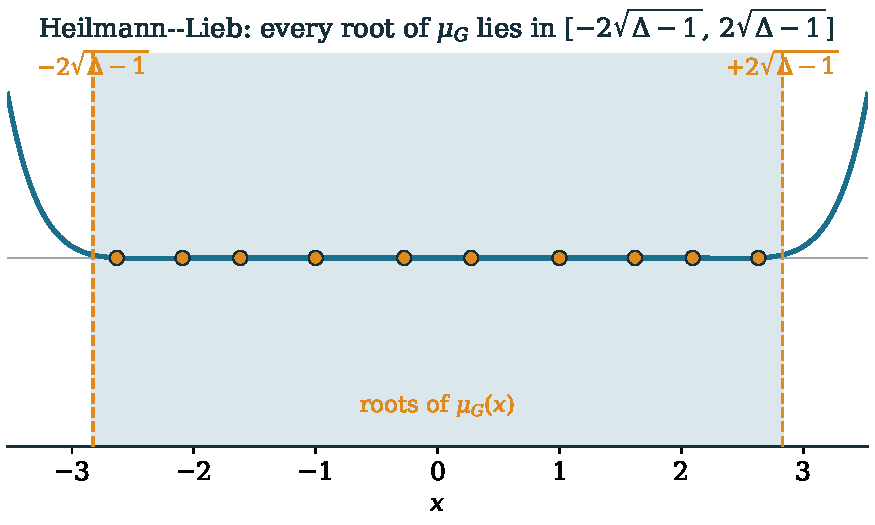
\includegraphics[width=0.92\textwidth]{fig1_band.pdf}
  \caption{El teorema, en una imagen. El polinomio de emparejamientos $\mu_G$
  (normalizado) del grafo de Petersen ($\Delta=3$), con sus ra\'ices (\'ambar) y la
  banda de Ramanujan $[-2\sqrt{\Delta-1},2\sqrt{\Delta-1}]$ sombreada.
  Heilmann--Lieb afirma---y \lean{matchingPoly\_bounded} ahora certifica---que las
  ra\'ices nunca abandonan la banda, para todo grafo finito con $\Delta\ge2$.}
  \label{fig:band}
\end{figure}

% ===============================================================
\section{Introducci\'on: una breve historia, y por qu\'e este art\'iculo}
\label{sec:history}

\emph{¿Podr\'ia un teorema nacido en la f\'isica de 1972, dotado de una
demostraci\'on puramente combinatoria en los a\~nos 80 y con un papel estelar
inesperado en 2015, ponerse por fin fuera de toda duda mediante una m\'aquina---y
para qu\'e servir\'ia?} Esa es la pregunta de fondo, y responderla exige que se
encuentren tres hilos de la historia.

El primer hilo es la \emph{mec\'anica estad\'istica}. En 1972, estudiando sistemas
mon\'omero--d\'imero---un gas reticular de d\'imeros que no se solapan---Heilmann y
Lieb~\cite{HeilmannLieb1972} demostraron que los ceros de la funci\'on de
partici\'on asociada evitan toda una regi\'on del plano complejo. Traducido a la
combinatoria, su resultado dice que el \emph{polinomio de emparejamientos}
$\mu_G(x)=\sum_k(-1)^k m_k x^{n-2k}$ de un grafo tiene solo ra\'ices reales, y que
esas ra\'ices quedan confinadas a la banda $[-2\sqrt{\Delta-1},\,2\sqrt{\Delta-1}]$
fijada por el grado m\'aximo $\Delta$. El resultado pertenece a la tradici\'on de
Lee--Yang (1952) de controlar un sistema f\'isico por la localizaci\'on de los ceros
de su funci\'on de partici\'on; la aportaci\'on de Heilmann y Lieb fue clavar esos
ceros al eje real y a un intervalo finito. El teorema naci\'o anal\'itico, en la
f\'isica, no en la teor\'ia de grafos.

El segundo hilo es la \emph{combinatoria}. En los a\~nos 80 Godsil dio una
demostraci\'on sin an\'alisis alguno~\cite{Godsil1981Matchings,Godsil1993}:
\emph{desplegar} el grafo $G$ en el \'arbol $T(G,u)$ de sus caminos, donde el
polinomio de emparejamientos coincide con el polinomio caracter\'istico de una
matriz sim\'etrica---de modo que la realidad y la banda son hechos espectrales---y
transportar la conclusi\'on de vuelta por la divisibilidad $\mu_G\mid\mu_{T(G,u)}$.
El borde de la banda $2\sqrt{\Delta-1}$ no es casualidad: es el radio espectral del
\'arbol $\Delta$-regular infinito, calculado por Kesten (1959), y es el n\'umero que
da nombre a los \emph{grafos de Ramanujan}. Esos expansores \'optimos---espectro no
trivial dentro de la banda---fueron construidos por Lubotzky, Phillips y Sarnak y
por Margulis (1988), cuya demostraci\'on de que la cota se alcanza descansaba en la
conjetura de Ramanujan--Petersson (de ah\'i el nombre); Alon--Boppana mostr\'o luego
que la cota no se puede mejorar asint\'oticamente. Vista de forma multiplicativa, la
misma banda es la l\'inea cr\'itica de la \emph{funci\'on zeta de Ihara} de un grafo
(Ihara 1966; Bass 1992): un grafo regular es de Ramanujan exactamente cuando su zeta
satisface un an\'alogo de la hip\'otesis de Riemann. Un solo n\'umero,
$2\sqrt{\Delta-1}$, enhebra emparejamientos, espectros y funciones zeta
(Figura~\ref{fig:km}).

\begin{figure}[t]
  \centering
  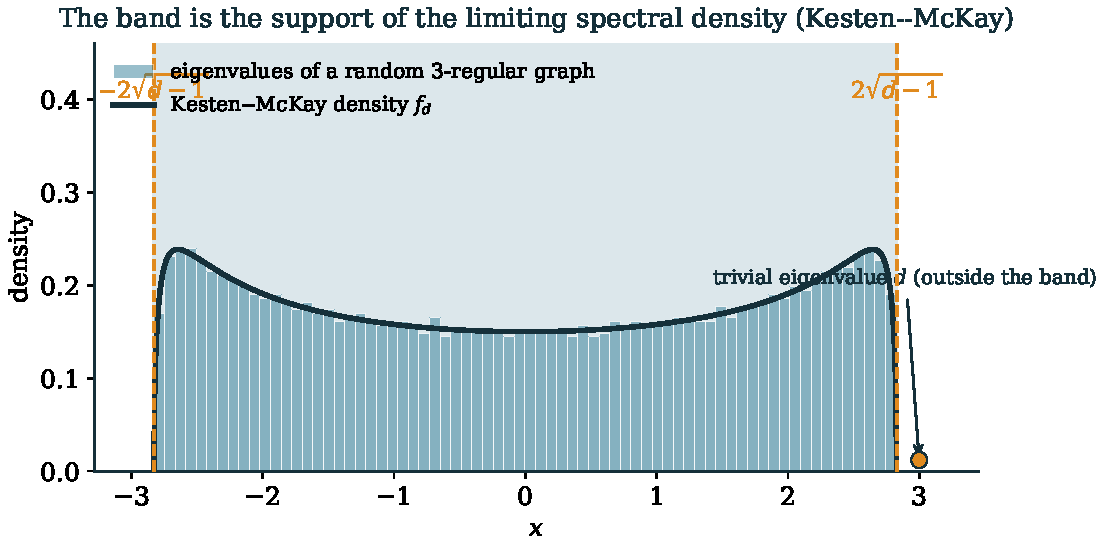
\includegraphics[width=0.9\textwidth]{fig6_kestenmckay.pdf}
  \caption{Por qu\'e $2\sqrt{\Delta-1}$ es el n\'umero correcto. Los autovalores de
  un grafo $3$-regular aleatorio (azul) siguen la densidad l\'imite de
  Kesten--McKay (curva oscura), y ambos viven exactamente en la banda
  $[-2\sqrt{d-1},\,2\sqrt{d-1}]$: la densidad alcanza los bordes (\'ambar) y se
  anula m\'as all\'a. El \'unico autovalor trivial $d$ queda fuera; un grafo es de
  \emph{Ramanujan} precisamente cuando todo autovalor no trivial permanece dentro
  de la banda---la misma banda en la que este art\'iculo confina las ra\'ices del
  polinomio de emparejamientos.}
  \label{fig:km}
\end{figure}

El tercer hilo es la \emph{inform\'atica te\'orica}. En 2015, Marcus, Spielman y
Srivastava~\cite{MSS2015a} demostraron que existen grafos de Ramanujan bipartitos de
todo grado---resolviendo una pregunta abierta de largo recorrido---y el motor
anal\'itico de su argumento es exactamente Heilmann--Lieb: el polinomio
caracter\'istico esperado de una matriz de adyacencia con signos aleatorios
\emph{es} el polinomio de emparejamientos (Godsil--Gutman), y sus ra\'ices est\'an
en la banda. Un teorema de la f\'isica de redes se hab\'ia convertido en la clave de
b\'oveda de un resultado famoso sobre redes de comunicaci\'on.

Frente a estos tres hilos se alza un cuarto, m\'as joven: el auge de los
\emph{asistentes de pruebas}. Sistemas como Lean y su biblioteca Mathlib soportan
hoy demostraciones verificadas por m\'aquina de matem\'atica moderna sustancial. Y
sin embargo---algo notable para un teorema tan central---ni el polinomio de
emparejamientos ni ninguna de las dos mitades de Heilmann--Lieb se hab\'ian
formalizado en ning\'un asistente de pruebas. El Paper~I~\cite{PartI} dio el primer
paso, formalizando el polinomio de emparejamientos y la identidad de
Godsil--Gutman, y propuso el \'arbol de caminos de Godsil como ruta hacia lo
dem\'as. \emph{Este art\'iculo recorre esa ruta hasta el final.} Lo que el lector
encontrar\'a es una demostraci\'on completa, \lean{sorry}-libre, verificada por
m\'aquina, de ambas mitades de Heilmann--Lieb, construida exactamente a lo largo del
despliegue de Godsil, con el \'unico muro de elaboraci\'on que hab\'ia detenido a un
borrador previo ya cruzado.

Por qu\'e importa es el encuentro de los hilos. Un Heilmann--Lieb verificado es un
enunciado de regi\'on libre de ceros sobre el que un f\'isico estad\'istico puede
construir; el insumo anal\'itico que un te\'orico de expansores necesita, ahora
fuera de duda; infraestructura reutilizable de raicicidad real y espectral para la
comunidad de matem\'atica formal; y un peldano concreto hacia una demostraci\'on
verificada de que los grafos de Ramanujan existen. La Secci\'on~\ref{sec:implications}
precisa el alcance entre campos, la Secci\'on~\ref{sec:context} dice claramente
d\'onde el teorema deja de ser \'util, y la Secci\'on~\ref{sec:open} deja sobre la
mesa las preguntas abiertas m\'as afiladas.

% ===============================================================
\section{El resultado}
\label{sec:intro}

Hasta aqu\'i el mapa; ahora el territorio. El Paper~I~\cite{PartI} termin\'o con una
promesa---\emph{``Si este art\'iculo tiene secuela, esta es su primera frase.''}---y
nombr\'o la ruta: demostrar Heilmann--Lieb no a trav\'es de la maquinaria de
familias entrelazadas, sino a trav\'es del \'arbol de caminos de Godsil, la \'unica
construcci\'on que entrega ambas mitades a la vez. Esta es esa frase, y el resto del
art\'iculo cumple la promesa.

El objeto de estudio es el \emph{polinomio de emparejamientos} de un grafo finito
$G$ con $n$ v\'ertices,
\keyeq{\mu_G(x)\;=\;\sum_{k\ge0}(-1)^k\,m_k\,x^{\,n-2k},}
donde $m_k$ es el n\'umero de emparejamientos de $k$ aristas de $G$ (y $m_0=1$).
Heilmann y Lieb~\cite{HeilmannLieb1972} demostraron dos hechos sobre sus ra\'ices:
son todas \emph{reales}, y todas est\'an en una banda cuya anchura fija solo el
grado m\'aximo $\Delta$.

\begin{theorem}[Heilmann--Lieb, en Lean~4]
\label{thm:HL}
Para todo grafo finito $G$, $\mu_G$ tiene todas sus ra\'ices reales
(\lean{matchingPoly\_realRooted}); y si $2\le\Delta$ y todo v\'ertice tiene grado
$\le\Delta$, entonces toda ra\'iz de $\mu_G$ est\'a en la banda
\keyeq{\bigl[-2\sqrt{\Delta-1},\;2\sqrt{\Delta-1}\bigr]\qquad
  (\lean{matchingPoly\_bounded}).}
Ambos enunciados son \lean{sorry}-libres; \lean{\#print axioms} sobre cada uno
reporta solo \lean{propext}, \lean{Classical.choice}, \lean{Quot.sound}.
\end{theorem}

La Figura~\ref{fig:band} muestra la conclusi\'on; la Tabla~\ref{tab:results} lista
cada ingrediente verificado; la Tabla~\ref{tab:numeric} confirma la cota
num\'ericamente en seis grafos.

\paragraph{La ruta, en un suspiro.}
Un \'arbol es f\'acil: en un bosque el polinomio de emparejamientos \emph{es igual}
al polinomio caracter\'istico de la matriz de adyacencia sim\'etrica, as\'i que sus
ra\'ices son reales, y el radio espectral de un \'arbol de grado m\'aximo $\Delta$
es a lo sumo $2\sqrt{\Delta-1}$. La idea de Godsil es reducir el grafo arbitrario a
este caso f\'acil \emph{desplegando}lo en el \'arbol $T(G,u)$ de sus caminos y
usando la divisibilidad
\keyeq{\mu_G \;\bigm|\; \mu_{T(G,u)}\qquad(\text{Godsil}),}
que transporta cualquier cota sobre las ra\'ices del \'arbol de vuelta a $G$. El
Paper~I nombr\'o exactamente estos dos hechos---divisibilidad e identidad del
bosque---como el trabajo pendiente. Este art\'iculo hace ambos, y demuestra la cota
espectral sobre el \'arbol desde cero.

\paragraph{Contribuciones.} Todo en Lean~4 / Mathlib, todo \lean{sorry}-libre
(Tabla~\ref{tab:results}):
\begin{enumerate}\itemsep2pt
\item \textbf{Raicicidad real} para todo grafo finito
  (\lean{matchingPoly\_realRooted}), v\'ia el \'arbol de caminos, su aciclicidad, la
  identidad del bosque y la divisibilidad $\mu_G\mid\mu_{T(G,u)}$---la \'ultima de
  las cuales requiri\'o cruzar un muro de elaboraci\'on que un borrador previo de
  este programa hab\'ia diagnosticado pero no superado (Secci\'on~\ref{sec:divis}).
\item \textbf{La cota de Ramanujan} para todo grafo finito con $\Delta\ge2$
  (\lean{matchingPoly\_bounded}), demostrada desde cero por una estimaci\'on de
  Gershgorin ponderado / Collatz--Wielandt (Secci\'on~\ref{sec:gershgorin})
  alimentada por un peso geom\'etrico de \'arbol y dos hechos sobre distancias en un
  \'arbol (Secci\'on~\ref{sec:weight}).
\item \textbf{Infraestructura reutilizable}: una cota de autovalores de Gershgorin
  ponderado, manejable y directa (\lean{collatzWielandt}); el predicado
  \lean{BoundedBy} cerrado bajo divisores y productos; y dos hechos limpios sobre
  distancias en \'arboles. Mathlib no ten\'ia ninguno, ni el polinomio de
  emparejamientos (Paper~I).
\end{enumerate}

\paragraph{Qu\'e afirmo como nuevo.} La matem\'atica es cl\'asica
(Secci\'on~\ref{sec:related}); la novedad est\'a en la formalizaci\'on y en algunas
cosas que tuve que construir o descubrir por el camino. Afirmo, en concreto:
\begin{enumerate}\itemsep1.5pt
\item[(N1)] la primera demostraci\'on verificada por m\'aquina de la que tengo
  constancia, en cualquier asistente, de \emph{ambas} mitades de Heilmann--Lieb---%
  raicicidad real y la cota de Ramanujan---y del polinomio de emparejamientos que
  conciernen (basada en b\'usqueda; v\'ease la salvedad m\'as abajo);
\item[(N2)] una cota de autovalores de Gershgorin ponderado, directa
  (\lean{collatzWielandt}), y el predicado \lean{BoundedBy} cerrado bajo divisores y
  productos---ninguno en Mathlib;
\item[(N3)] dos lemas reutilizables sobre distancias en \'arboles---los vecinos
  difieren en distancia-al-raíz por exactamente uno, y a lo sumo un vecino est\'a
  m\'as cerca---demostrados respectivamente desde la bipartici\'on y la unicidad de
  caminos;
\item[(N4)] el cruce del muro de elaboraci\'on que hab\'ia detenido al borrador de
  \'arboles de caminos de este programa, con el diagn\'ostico exacto (divergencia de
  instancias sobre el tipo $\Sigma$ de caminos) y su cura (una reescritura de
  irrelevancia de instancia con la cabeza fijada);
\item[(N5)] un peso de prueba \emph{local} en las aristas que telescopia a la cota
  m\'as fina por arista $\sqrt{d_u-1}+\sqrt{d_v-1}$ y es el objeto m\'as limpio de
  formalizar;
\item[(N6)] un negativo honesto documentado---el manejo bilateral
  $\mathbb{E}[\operatorname{charpoly}(A_s^2)]$ \emph{no} tiene ra\'ices reales---que
  cierra una ruta tentadora hacia el problema abierto de Ramanujan no bipartito.
\end{enumerate}
Soy cuidadoso con el tipo de novedad: (N1)--(N4) son contribuciones de
\emph{formalizaci\'on}, (N5) una cota de tipo conocido que creo verificada por
m\'aquina por primera vez, y (N6) un resultado negativo; ninguna es matem\'atica
nueva en el sentido de demostrar un teorema, y las separo del contenido cl\'asico
deliberadamente.

\paragraph{Y, sin rodeos, qu\'e no es.} Es una formalizaci\'on de matem\'atica
cl\'asica; no demuestra ning\'un teorema nuevo y no lo pretende. La cota necesita
$\Delta\ge2$ y no demuestro que baste algo m\'as d\'ebil, exhibiendo d\'onde falla
(Secci\'on~\ref{sec:weight}). Y ``primera formalizaci\'on'' se apoya en una
b\'usqueda en los tres ecosistemas mayores de asistentes de pruebas---Lean/Mathlib,
el Archivo de Pruebas Formales de Isabelle y Coq/mathcomp---en ninguno de los cuales
parece estar el polinomio de emparejamientos ni ninguna mitad de Heilmann--Lieb
(Mathlib tiene \lean{IsMatching} pero no el polinomio de emparejamientos). Es una
b\'usqueda en cat\'alogos y archivos de discusi\'on, no una auditor\'ia byte a byte
de toda biblioteca, y lo enuncio como exactamente eso.

% Tablas a color para el documento Heilmann--Lieb (Paper II), versión española.
% Requiere: \usepackage[table]{xcolor}; colores ggteal, ggband, ggamber en el preámbulo.

\begin{table}[t]
\centering
\renewcommand{\arraystretch}{1.25}
\setlength{\tabcolsep}{7pt}
\rowcolors{2}{ggband}{white}
\begin{tabular}{@{}>{\raggedright\arraybackslash}p{0.345\textwidth} >{\raggedright\arraybackslash}p{0.46\textwidth} c@{}}
\rowcolor{ggteal}
\textcolor{white}{\bf Teorema en Lean} & \textcolor{white}{\bf Enunciado} & \textcolor{white}{\bf sin \lean{sorry}} \\
\lean{matchingPoly\_realRooted} & $\mu_G$ tiene todas sus raíces reales, todo $G$ finito & \checkmark \\
\lean{matchingPoly\_bounded} & raíces de $\mu_G$ en $[-2\sqrt{\Delta-1},2\sqrt{\Delta-1}]$ ($2\le\Delta$, $\deg\le\Delta$) & \checkmark \\
\lean{connected\_matchingPoly\_dvd\_pathTree} & $\mu_G \mid \mu_{T(G,u)}$ (divisibilidad, ladrillo) & \checkmark \\
\lean{matchingPoly\_forest\_eq\_charpoly} & $\mu_F=\operatorname{charpoly}(A_F)$ en un bosque & \checkmark \\
\lean{collatzWielandt} & cota de autovalores tipo Gershgorin ponderado & \checkmark \\
\lean{forest\_bounded\_proof} & raíces del matching de un bosque en la banda & \checkmark \\
\lean{forest\_adj\_dist\_pm\_one} & vecinos difieren en distancia-al-raíz por $1$ & \checkmark \\
\lean{forest\_le\_one\_parent} & $\le 1$ vecino más cerca del raíz & \checkmark \\
\lean{pathTree\_degree\_le} & $\deg T(G,u)\le \deg G$ & \checkmark \\
\end{tabular}
\caption{Los resultados verificados por máquina de este artículo, en Lean~4 / Mathlib. Cada
entrada es \lean{sorry}-libre; \lean{\#print axioms} sobre cada una reporta solo \lean{propext},
\lean{Classical.choice}, \lean{Quot.sound} (sin \lean{sorryAx}). Cadena de herramientas
\lean{leanprover/lean4:v4.30.0-rc2}, clon local de Mathlib; verificado con \lean{lake build MSS}
(salida~0).}
\label{tab:results}
\end{table}

\begin{table}[t]
\centering
\renewcommand{\arraystretch}{1.25}
\setlength{\tabcolsep}{9pt}
\rowcolors{2}{ggband}{white}
\begin{tabular}{@{}l c c c c c@{}}
\rowcolor{ggteal}
\textcolor{white}{\bf grafo $G$} & \textcolor{white}{$n$} & \textcolor{white}{$\Delta$} &
\textcolor{white}{$2\sqrt{\Delta-1}$} & \textcolor{white}{$\max_i|\rho_i|$} & \textcolor{white}{en banda} \\
camino $P_6$       & 6 & 2 & 2.0000 & 1.8019 & \checkmark \\
ciclo $C_6$        & 6 & 2 & 2.0000 & 1.9319 & \checkmark \\
estrella $K_{1,5}$ & 6 & 5 & 4.0000 & 2.2361 & \checkmark \\
completo $K_5$     & 5 & 4 & 3.4641 & 2.8570 & \checkmark \\
Petersen           & 10 & 3 & 2.8284 & 2.6314 & \checkmark \\
cubo $Q_3$         & 8 & 3 & 2.8284 & 2.5779 & \checkmark \\
\end{tabular}
\caption{Confirmación numérica de la cota (\lean{matchingPoly\_bounded}). Para cada grafo,
$\Delta$ es el grado máximo, $2\sqrt{\Delta-1}$ el borde de la banda de Ramanujan, y
$\max_i|\rho_i|$ la mayor magnitud entre las raíces $\rho_i$ de $\mu_G$ (calculadas exactamente).
Todo valor cumple $\max_i|\rho_i|\le 2\sqrt{\Delta-1}$. Calculado en SageMath.}
\label{tab:numeric}
\end{table}


% ===============================================================
\section{¿Qu\'e es el \'arbol de caminos?}
\label{sec:pathtree}

¿C\'omo puede reducirse un enunciado sobre un grafo \emph{arbitrario}---con todos
sus ciclos---a un enunciado sobre \'arboles? La respuesta de Godsil es reemplazar
$G$ por un \'arbol que ``ve'' los mismos emparejamientos: el \'arbol de todos los
caminos.

\begin{definition}[\'Arbol de caminos]
\label{def:pathtree}
Para un grafo finito $G$ y un v\'ertice $u$, sea
$\mathrm{PathFrom}\,G\,u=\Sigma_{v}\,G.\mathrm{Path}\,u\,v$ el tipo de los caminos
simples de $G$ que empiezan en $u$. El \emph{\'arbol de caminos}
$T(G,u)=\lean{pathTree}\,G\,u$ es el \lean{SimpleGraph} sobre este tipo en el que
dos caminos son adyacentes cuando uno extiende al otro por una sola arista a\~nadida
al final (la relaci\'on \lean{Grows}). El raíz $r$ es el camino trivial en $u$.
\end{definition}

Lo primero por demostrar es que el nombre es honesto.

\begin{theorem}[Es un bosque]
\label{thm:acyclic}
$T(G,u)$ es ac\'iclico (\lean{pathTree\_isAcyclic}).
\end{theorem}

La demostraci\'on rota un ciclo hipot\'etico hasta un v\'ertice $m$ de longitud de
camino m\'axima; sus dos vecinos en el ciclo son m\'as cortos, as\'i que ambos
\emph{crecen hacia} $m$, es decir, ambos son su padre (el camino con la \'ultima
arista quitada). Los padres son \'unicos---un \lean{Walk.concat} es inyectivo en su
\'ultima arista (\lean{Grows.parent\_unique})---as\'i que los dos vecinos coinciden,
contradiciendo que los dos vecinos de un v\'ertice en un ciclo son distintos. La
Figura~\ref{fig:pathtree} muestra un caso peque\~no.

\begin{figure}[t]
  \centering
  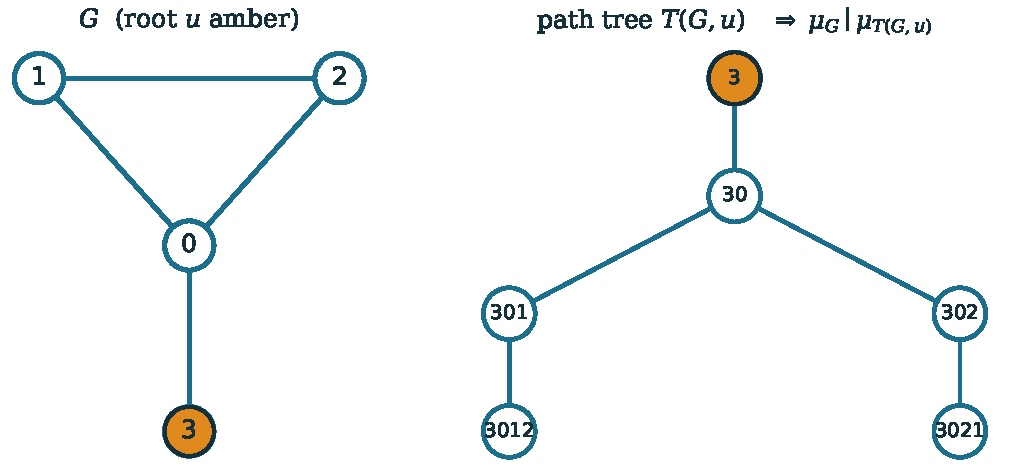
\includegraphics[width=0.96\textwidth]{fig2_pathtree.pdf}
  \caption{Desplegando el grafo ``pata'' $G$ (izquierda, raíz $u$ en \'ambar) en su
  \'arbol de caminos $T(G,u)$ (derecha): cada v\'ertice de $T$ es un camino simple
  de $G$ desde $u$, escrito como su sucesi\'on de v\'ertices; dos se unen cuando uno
  extiende al otro por una arista. $T(G,u)$ es ac\'iclico (Teorema~\ref{thm:acyclic}),
  y $\mu_G$ divide a $\mu_{T(G,u)}$ (Secci\'on~\ref{sec:divis}).}
  \label{fig:pathtree}
\end{figure}

% ===============================================================
\section{Hecho (ii): los bosques son gauge-triviales}
\label{sec:forest}

¿Por qu\'e un \'arbol es el caso f\'acil? Porque en \'el el polinomio de
emparejamientos pierde su car\'acter combinatorio y se vuelve un objeto espectral.

\begin{theorem}[Identidad del bosque]
\label{thm:forest}
Para un grafo ac\'iclico $F$,
\keyeq{\mu_F \;=\; \operatorname{charpoly}(A_F)\qquad
  (\lean{matchingPoly\_forest\_eq\_charpoly}),}
el polinomio caracter\'istico de la matriz de adyacencia (real, sim\'etrica).
\end{theorem}

La demostraci\'on es la expansi\'on por permutaciones de $\det(xI-A_F)$. Una
permutaci\'on contribuye solo a trav\'es de su soporte; en un bosque, el soporte de
toda permutaci\'on contribuyente se descompone en transposiciones a lo largo de
aristas---el \emph{lema de involuci\'on del bosque}
(\lean{acyclic\_perm\_support\_isInvolution}): toda permutaci\'on cuyo punto no fijo
es adyacente a su imagen es una involuci\'on, porque una \'orbita m\'as larga
cerrar\'ia un ciclo. Los t\'erminos supervivientes son exactamente los
emparejamientos, con los signos correctos, reensamblando $\mu_F$. Como $A_F$ es real
sim\'etrica, el teorema espectral da espectro real
(\lean{charpoly\_symmetric\_realRooted}): $\mu_F$ tiene ra\'ices reales. El hecho
espectral m\'as dif\'icil---que las ra\'ices est\'an en la banda---es todo el
contenido de las Secciones~\ref{sec:gershgorin}--\ref{sec:weight}.

% ===============================================================
\section{Hecho (i): la divisibilidad, y el muro que cruc\'e}
\label{sec:divis}

Un \'arbol es f\'acil, pero el polinomio que me importa vive en $G$, no en
$T(G,u)$. As\'i que la pregunta afilada es: \emph{¿por qu\'e el polinomio de
emparejamientos de un grafo arbitrario---ciclos incluidos---deber\'ia dividir al de
un \'arbol construido a partir de sus caminos?} La identidad del bosque hace al
\'arbol f\'acil; la divisibilidad lo hace \emph{relevante}.

\begin{theorem}[Divisibilidad]
\label{thm:divis}
Para un grafo conexo $G$ y un v\'ertice $u$,
\keyeq{\mu_G \;\bigm|\; \mu_{T(G,u)}\qquad
  (\lean{connected\_matchingPoly\_dvd\_pathTree}).}
\end{theorem}

Matem\'aticamente esto es la inducci\'on de Godsil sobre la recurrencia de borrado
de v\'ertice del polinomio de emparejamientos,
\keyeq{\mu_G \;=\; x\,\mu_{G-v}\;-\;\sum_{u\sim v}\mu_{G-v-u}
  \qquad(\lean{matchingPoly\_recurrence}),}
aplicada en $u$ en $G$ y en el raíz $r$ en $T$, y combinada mediante la
\emph{identidad de Godsil}
\keyeq{\mu_G\,\mu_{T(G,u)-r}\;=\;\mu_{G-u}\,\mu_{T(G,u)},}
que, con la descomposici\'on en el raíz del \'arbol de caminos, da la divisibilidad.
(La formalizaci\'on lleva la recurrencia en su forma despejada por $x^2$, aislando
un v\'ertice en cada borrado, para mantener fijo el n\'umero de v\'ertices.) Lo que
merece relatarse es el \'ultimo paso, porque es donde un borrador previo de este
art\'iculo se detuvo.

\paragraph{El muro.} El \'arbol de caminos vive sobre un tipo dependiente $\Sigma$
de caminos. Especializar la divisibilidad general a un grafo concreto exige a Lean
comparar el polinomio de emparejamientos calculado con una instancia de
\lean{Fintype}/\lean{DecidableRel} contra el mismo polinomio calculado con otra; los
dos son \emph{iguales} (el polinomio no depende de estas instancias subsingleton),
pero pedir a \lean{isDefEq} que lo vea fuerza una reducci\'on \lean{whnf} de $\mu$
sobre el tipo de caminos, y el presupuesto de \emph{heartbeats} se agota. El
borrador lo diagnostic\'o como un muro de \emph{elaboraci\'on}, no una laguna
matem\'atica, y se detuvo ah\'i.

\paragraph{El cruce.} La cura es transportar la \emph{hip\'otesis} a las instancias
locales en vez del objetivo a las for\'aneas. Con el lema de irrelevancia de
instancia \lean{matchingPoly\_inst\_irrel} (demostrado con \lean{Subsingleton.elim},
no con \lean{congr}, precisamente para evitar el \lean{whnf}), se reescribe cada
aparici\'on de $\mu(T(G,u))$ con la \emph{cabeza del grafo fijada}, haciendo de la
reescritura un emparejamiento sint\'actico que nunca reduce $\mu$. Cuatro
reescrituras as\'i cierran el teorema; \lean{\#print axioms} no reporta
\lean{sorryAx}. La lecci\'on que el borrador solo pod\'ia conjeturar queda ahora
confirmada en c\'odigo: el muro era divergencia de instancias, y fijar la cabeza lo
disuelve.

% ===============================================================
\section{Raicicidad real, ensamblada}
\label{sec:realrooted}

La divisibilidad (Teorema~\ref{thm:divis}) necesita $G$ conexo; \emph{¿lo necesita
la raicicidad real?} No---y la brecha es justo la uni\'on disjunta, que el polinomio
de emparejamientos resuelve multiplicando. Con los dos hechos en la mano, la
raicicidad real es corta. Un divisor no nulo de un polinomio que escinde sobre $\R$
tambi\'en escinde (\lean{RealRooted.of\_dvd}, envolviendo
\lean{Polynomial.Splits.of\_dvd}). El \'arbol de caminos es un bosque
(Teorema~\ref{thm:acyclic}), as\'i que $\mu_{T(G,u)}$ es un polinomio
caracter\'istico de una matriz sim\'etrica, luego escinde (Teorema~\ref{thm:forest});
por tanto su divisor $\mu_G$ tambi\'en---$\mu_G$ tiene ra\'ices reales para $G$
conexo (\lean{matchingPoly\_connected\_realRooted}). Un grafo general es la uni\'on
disjunta de sus componentes y $\mu$ es multiplicativo sobre componentes
(\lean{matchingPoly\_eq\_prod\_components}); cada componente inducida es conexa
(\lean{maximal\_connected\_induce\_supp}), y la raicicidad real multiplica. Esto es
\lean{matchingPoly\_realRooted}, para todo grafo finito.

% ===============================================================
\section{La cota, primera mitad: una estimaci\'on de Gershgorin ponderado}
\label{sec:gershgorin}

La raicicidad real dice que las ra\'ices son reales; la cota dice que ninguna excede
un techo fijado solo por el grado. ¿De d\'onde sale un techo dependiente solo del
grado sobre el mayor autovalor de una matriz sim\'etrica?

La herramienta es una estimaci\'on de Gershgorin \emph{ponderada}---la direcci\'on
de Collatz--Wielandt de Perron--Frobenius, enunciada para un autovalor y demostrada
a mano para no necesitar teor\'ia de positividad.

\begin{theorem}[Gershgorin ponderado]
\label{thm:cw}
Sea $A$ una matriz real cuadrada con entradas no negativas y $w$ un vector
estrictamente positivo con $\sum_j A_{ij}\,w_j\le B\,w_i$ para todo $i$. Entonces
toda ra\'iz real $\mu$ de $\operatorname{charpoly}(A)$ cumple
\keyeq{|\mu|\;\le\;B\qquad(\lean{collatzWielandt}).}
\end{theorem}

La demostraci\'on es el argumento del autovector y el \'indice de m\'aximo, y es lo
bastante corta para darla entera. Una ra\'iz del polinomio caracter\'istico da, por
$\det(\mu I-A)=0$ y \lean{Matrix.exists\_mulVec\_eq\_zero\_iff}, un autovector
$v\ne0$ con $Av=\mu v$. Elige la coordenada $k$ que maximiza $|v_j|/w_j$. Entonces,
usando $A_{kj}\ge0$ y $|v_j|/w_j\le|v_k|/w_k$,
\[
  |\mu|\,|v_k|
  =\Bigl|\sum_j A_{kj}v_j\Bigr|
  \le\sum_j A_{kj}\,w_j\frac{|v_j|}{w_j}
  \le\Bigl(\sum_j A_{kj}w_j\Bigr)\frac{|v_k|}{w_k}
  \le B\,w_k\frac{|v_k|}{w_k}=B\,|v_k|,
\]
y $|v_k|>0$. Este es todo el motor anal\'itico de la cota. Pegarlo al polinomio de
emparejamientos es un lema (\lean{forest\_bounded\_of\_weight}): en un bosque, $A_F$
es sim\'etrica y no negativa (sus entradas son $0/1$) y $\mu_F$ es su polinomio
caracter\'istico (Teorema~\ref{thm:forest}), as\'i que el Teorema~\ref{thm:cw} acota
las ra\'ices---\emph{una vez que exhiba un peso cuyas sumas de fila ponderadas sean
$\le 2\sqrt{\Delta-1}$}.

% ===============================================================
\section{La cota, segunda mitad: un peso y dos hechos de \'arbol}
\label{sec:weight}

¿Qu\'e peso fuerza las sumas de fila justo hasta $2\sqrt{\Delta-1}$? En un \'arbol,
con raíz en un v\'ertice por componente, da a cada v\'ertice un peso que decae
geom\'etricamente con su distancia al raíz:
\keyeq{w_v\;=\;\bigl(\sqrt{\Delta-1}\bigr)^{-\operatorname{dist}(r,v)}.}
La aritm\'etica de por qu\'e funciona es el contenido de la
Figura~\ref{fig:weight}. Escribe $s=\sqrt{\Delta-1}$ y $q=\Delta-1$. Un vecino un
paso \emph{m\'as cerca} del raíz aporta $w_v\cdot s$; uno un paso \emph{m\'as lejos}
aporta $w_v/s$. As\'i, con $a$ vecinos m\'as cercanos y $b$ m\'as lejanos,
\[
  \sum_{u\sim v}w_u \;=\; w_v\Bigl(a\,s+\tfrac{b}{s}\Bigr),
\]
y la cota $a\,s+b/s\le 2s$ se reduce, tras multiplicar por $s$ y usar $s^2=q$, a una
sola desigualdad entera:
\keyeq{a\,q+b\;\le\;2q,\qquad\text{es decir}\qquad (\Delta-2)(1-a)\ge0,}
que se cumple con $a\le1$ (Hecho~2 abajo), $a+b\le\Delta$ (la cota de grado) y
$\Delta\ge2$. Esta \'ultima aritm\'etica se a\'isla como \lean{rowsum\_arith}, y es
donde la hip\'otesis $\Delta\ge2$ se gana su lugar.

\begin{figure}[t]
  \centering
  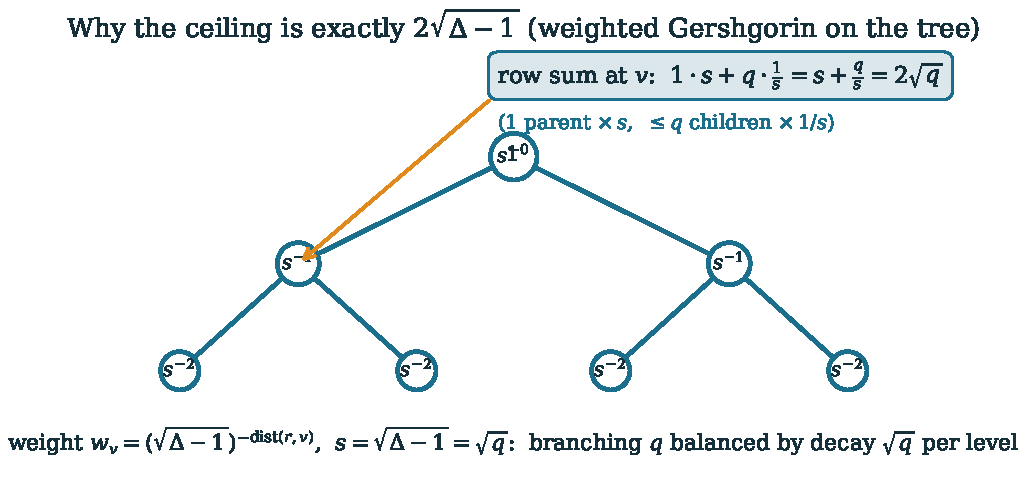
\includegraphics[width=0.92\textwidth]{fig3_weight.pdf}
  \caption{Por qu\'e el techo es exactamente $2\sqrt{\Delta-1}$. Con el peso
  geom\'etrico $w_v=(\sqrt{\Delta-1})^{-\operatorname{dist}(r,v)}$, la suma de fila
  ponderada en un v\'ertice $v$ equilibra su \'unico padre (m\'as pesado por
  $s=\sqrt{q}$) contra sus $\le q$ hijos (m\'as ligeros por $s$), dando
  $s+q/s=2\sqrt{q}$. El factor de ramificaci\'on $q$ queda exactamente cancelado por
  un decaimiento $\sqrt{q}$ por nivel.}
  \label{fig:weight}
\end{figure}

Los dos insumos estructurales que consume el c\'omputo de la suma de fila son toda
la teor\'ia de grafos que la cota necesita de verdad. Ambos son hechos sobre
distancias al raíz en un \'arbol.

\begin{theorem}[Hecho 1: los vecinos difieren por exactamente uno]
\label{thm:f1}
En un grafo ac\'iclico con raíz $\rho$, para una arista $u\sim v$ con $u$ alcanzable
desde $\rho$, $\operatorname{dist}(\rho,u)=\operatorname{dist}(\rho,v)\pm1$
(\lean{forest\_adj\_dist\_pm\_one}).
\end{theorem}

La mitad $\le1$ es la desigualdad triangular: un camino m\'as corto a un extremo,
extendido por la arista, alcanza el otro. La mitad $\ne$ es la bipartici\'on. Un
\'arbol es bipartito (\lean{IsAcyclic.isBipartite}), as\'i que existe una
$2$-coloraci\'on $c$; sobre un camino m\'as corto, $c$ registra la paridad de su
longitud (\lean{Coloring.even\_length\_iff\_congr}), de modo que el color de un
v\'ertice es la paridad de su distancia a $\rho$. Los v\'ertices adyacentes tienen
colores distintos (\lean{Coloring.valid}), luego paridades distintas, luego
distancias distintas.

\begin{theorem}[Hecho 2: a lo sumo un padre]
\label{thm:f2}
En un grafo ac\'iclico, a lo sumo un vecino de $v$ est\'a un paso m\'as cerca del
raíz (\lean{forest\_le\_one\_parent}).
\end{theorem}

Dos vecinos as\'i dar\'ian dos caminos m\'as cortos $\rho\to v$ terminando en
\'ultimas aristas distintas; en un \'arbol el camino entre dos v\'ertices es \'unico
(\lean{IsAcyclic.path\_unique}), y \lean{IsPath.eq\_penultimate\_of\_mem\_edges}
fija ambos candidatos al \'unico v\'ertice pen\'ultimo de ese camino, as\'i que
coinciden. (Un paseo m\'as corto es un camino---v\'ia \lean{bypass}---provee los
caminos m\'as cortos: \lean{exists\_isPath\_length\_eq\_dist}.)

Ensamblando el peso, los dos hechos y la aritm\'etica se obtiene la cota del bosque
(\lean{forest\_bounded\_proof}): \emph{el polinomio de emparejamientos de un bosque
de grado m\'aximo $\le\Delta$ tiene todas sus ra\'ices en
$[-2\sqrt{\Delta-1},2\sqrt{\Delta-1}]$.} Como $\mu_F=\operatorname{charpoly}$, esto
es exactamente el enunciado cl\'asico de que un \'arbol de grado m\'aximo $\Delta$
tiene radio espectral $\le2\sqrt{\Delta-1}$ (Godsil; Stevanovi\'c~\cite{Stevanovic2003})
---ahora, hasta donde s\'e, verificado por una m\'aquina por primera vez.

\paragraph{Un peso m\'as fino, local.} El peso anterior usa el $\Delta$ global. Una
elecci\'on puramente \emph{local}---multiplicar por $1/\sqrt{d_{\text{padre}}-1}$ en
cada paso al bajar del raíz---telescopia a la cota por arista
$\sqrt{d_u-1}+\sqrt{d_v-1}$, estrictamente m\'as fina en \'arboles irregulares y
recuperando $2\sqrt{\Delta-1}$ en el caso regular (confirmado num\'ericamente antes
de formalizar). Es el objeto m\'as limpio---definido localmente por arista, sin
necesidad de profundidad global---y es la forma que usa el desarrollo. No afirmo la
cota local como matem\'atica nueva: las cotas espectrales por sucesi\'on de grados
para \'arboles est\'an bien estudiadas; la aportaci\'on es el enunciado verificado.

\paragraph{La frontera, dicha con honestidad.} La hip\'otesis $\Delta\ge2$ no es
cosm\'etica. En $\Delta=1$ la banda $2\sqrt{\Delta-1}$ colapsa a $\{0\}$, pero una
sola arista $K_2$ tiene $\mu_{K_2}=x^2-1$ con ra\'ices $\pm1$. (Para $\Delta\le1$ un
grafo es un emparejamiento, con ra\'ices en $\{-1,0,1\}$.) Es la hip\'otesis
est\'andar de Heilmann--Lieb; la se\~nalo porque solo la advert\'i probando el caso
frontera, y una formalizaci\'on honesta debe decir d\'onde su enunciado es falso.

% ===============================================================
\section{Ensamblaje: del \'arbol a todo grafo}
\label{sec:assembly}

La cota ya vale en $T(G,u)$---un grafo cuyos v\'ertices son \emph{caminos}, no los
v\'ertices de $G$. \emph{¿Qu\'e se interpone entre esa cota y la que quiero en $G$?}
Tres pasos cortos, y son exactamente la brecha.

\textbf{El \'arbol de caminos no es demasiado frondoso} (\lean{pathTree\_degree\_le}):
$T(G,u)$ tiene grado m\'aximo $\le\Delta_G$. La aplicaci\'on ``un vecino del \'arbol
de caminos $\mapsto$ su extremo'' inyecta los vecinos de un nodo $p$ en los vecinos
en $G$ del extremo de $p$; la inyectividad es la estructura del \'arbol de
caminos---los hijos est\'an determinados por su extremo, el padre es \'unico, y un
hijo y el padre no pueden compartir extremo.

\textbf{Transporte} (\lean{connected\_matchingPoly\_bounded}): por el
Teorema~\ref{thm:divis}, $\mu_G\mid\mu_{T(G,u)}$, y el \'arbol de caminos es un
bosque de grado $\le\Delta$, as\'i que su polinomio de emparejamientos est\'a en la
banda (\lean{forest\_bounded\_proof}); un divisor no nulo de un polinomio en banda
est\'a en banda (\lean{BoundedBy.of\_dvd}). El transporte topa con el mismo muro
\lean{whnf} de los caminos $\Sigma$ que la divisibilidad, y la misma cirug\'ia
\lean{matchingPoly\_inst\_irrel} lo disuelve---esta vez la compilaci\'on termina sin
ning\'un \emph{timeout}.

\textbf{General} (\lean{matchingPoly\_bounded}): sobre componentes conexas
(\lean{BoundedBy.prod}), con cada componente inducida conexa y de grado
$\le\Delta$---sus vecinos en $G$ permanecen dentro de la componente, as\'i que
\lean{degree\_induce\_of\_neighborSet\_subset} da igualdad. Esta es la cota del
Teorema~\ref{thm:HL}. La Figura~\ref{fig:nested} muestra la cadena de contenciones
que la demostraci\'on realiza; la Tabla~\ref{tab:numeric} confirma el extremo
num\'ericamente.

\begin{figure}[t]
  \centering
  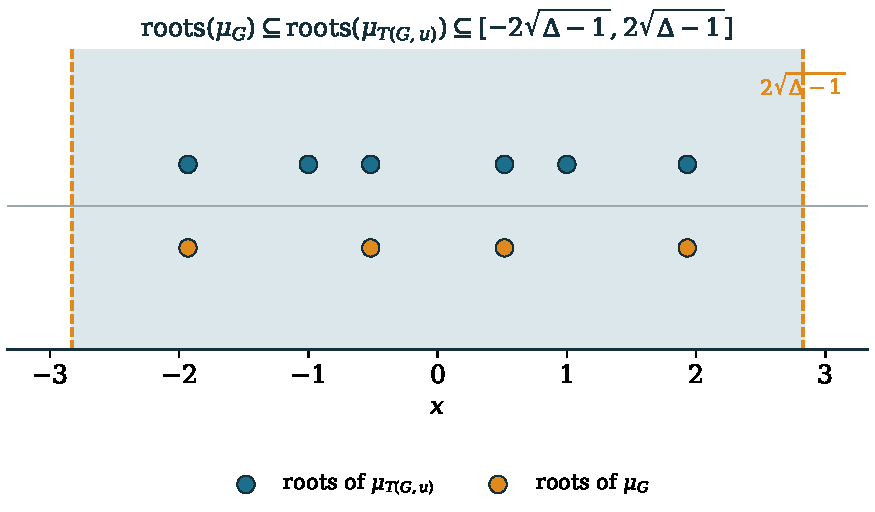
\includegraphics[width=0.88\textwidth]{fig4_nested.pdf}
  \caption{La demostraci\'on en una l\'inea de razonamiento, sobre el grafo pata:
  las ra\'ices de $\mu_G$ son un subconjunto de las de $\mu_{T(G,u)}$ (porque
  $\mu_G\mid\mu_{T(G,u)}$), que est\'an en la banda (porque $T(G,u)$ es un bosque).
  Luego las ra\'ices de $\mu_G$ est\'an en la banda.}
  \label{fig:nested}
\end{figure}

% ===============================================================
\section{Por qu\'e una sola construcci\'on da ambas mitades}
\label{sec:duality}

La raicicidad real y la cota parecen dos teoremas---uno sobre realidad, otro sobre
magnitud. \emph{¿Por qu\'e un solo \'arbol resuelve ambos a la vez?} Un hilo corto
lo explica, y ata este art\'iculo al lado de la zeta de Ihara del mismo programa.
Considera el cociente $R(G,a)=\mu_{G-a}/\mu_G$, la funci\'on de Green del polinomio
de emparejamientos. Dividir la recurrencia de borrado por $\mu_{G-a}$ la convierte en
una fracci\'on continua $1/R_a=x-\sum_{b\sim a}R_b$; en el \'arbol $(q{+}1)$-regular
esto es autoconsistente y resuelve $qR^2-xR+1=0$, cuya rama es $R=1/u$ con $u$ la
variable no retrocedente de Ihara. Las variables espectral y zeta se atan por el
mapa de Joukowski
\keyeq{\lambda \;=\; u+\frac{q}{u}\;=\;q\,R+\frac1R ,\qquad q=\Delta-1.}
En el c\'irculo cr\'itico $|u|=1/\sqrt{q}$ esto da $\lambda=2\sqrt{q}\,\cos\theta$:
la banda $[-2\sqrt{q},2\sqrt{q}]$ es precisamente la \emph{sombra} del c\'irculo
cr\'itico bajo Joukowski, una proyecci\'on dos a uno que identifica los pares
conjugados $u,\bar u$ (Figura~\ref{fig:joukowski}). La raicicidad real de $\mu_G$ es
el enunciado de que $R$ es una funci\'on de Stieltjes; la cota es la localizaci\'on
de su corte de rama. Verifiqu\'e el \'algebra simb\'olicamente y no la afirmo como
nueva (es la funci\'on de Green del ret\'iculo de Bethe / Kesten--McKay encontrando
el cuadro de Ihara--Bass); es la raz\'on de que el \'arbol de caminos y la funci\'on
zeta de un grafo, formalizados en el mismo repositorio, sean dos lecturas de una
variable.

\begin{figure}[t]
  \centering
  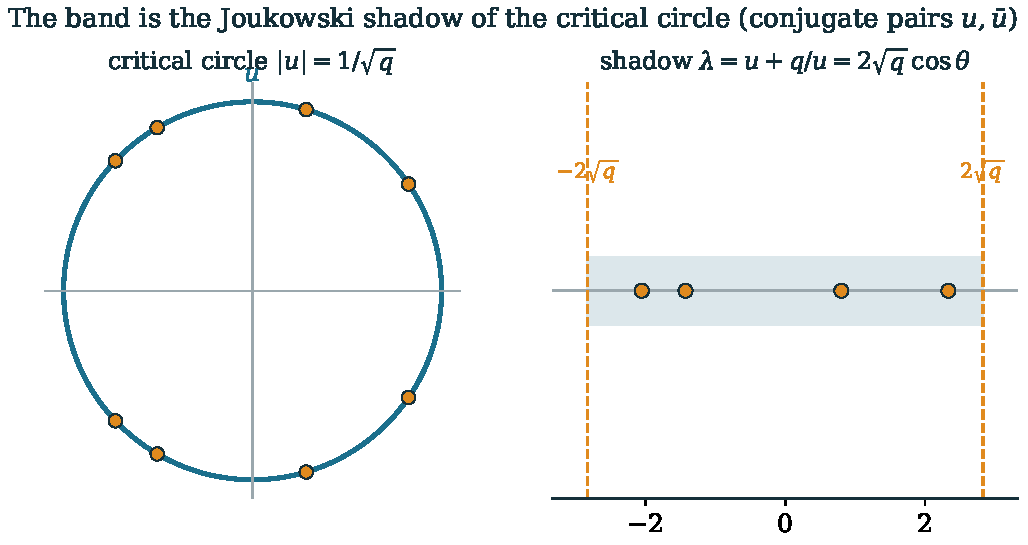
\includegraphics[width=0.92\textwidth]{fig5_joukowski.pdf}
  \caption{La banda es la sombra de Joukowski del c\'irculo cr\'itico. Los puntos
  $u,\bar u$ del c\'irculo $|u|=1/\sqrt{q}$ (izquierda) se proyectan a un solo
  $\lambda=u+q/u=2\sqrt{q}\cos\theta$ real en la banda $[-2\sqrt{q},2\sqrt{q}]$
  (derecha). La identificaci\'on dos a uno de conjugados es la ecuaci\'on funcional
  de la zeta de Ihara disfrazada.}
  \label{fig:joukowski}
\end{figure}

% ===============================================================
\section{Para qu\'e sirve el teorema, y para qu\'e no}
\label{sec:context}

Una afirmaci\'on verificada por m\'aquina merece una pregunta directa: \emph{¿qu\'e
puede hacer que el teorema informal no pudiera, y d\'onde acaba su alcance?}
Heilmann--Lieb es el insumo anal\'itico de la demostraci\'on de Marcus--Spielman--%
Srivastava de que existen grafos de Ramanujan bipartitos de todo
grado~\cite{MSS2015a}. Su argumento necesita dos hechos sobre el polinomio
caracter\'istico esperado de un signado $\pm1$ aleatorio de aristas: que es igual a
$\mu_G$ (Godsil--Gutman, Paper~I), y que sus ra\'ices est\'an en la banda
(Teorema~\ref{thm:HL}). \emph{Ambos est\'an ahora formalizados}
(Figura~\ref{fig:interlacing}). Lo que no est\'a aqu\'i es el paso de existencia de
las familias entrelazadas, ni la correspondencia signado/$2$-recubrimiento; eso
queda como trabajo futuro, y no afirmo nada sobre ello. En particular, este
art\'iculo formaliza Heilmann--Lieb, no la existencia de grafos de Ramanujan.

\begin{figure}[t]
  \centering
  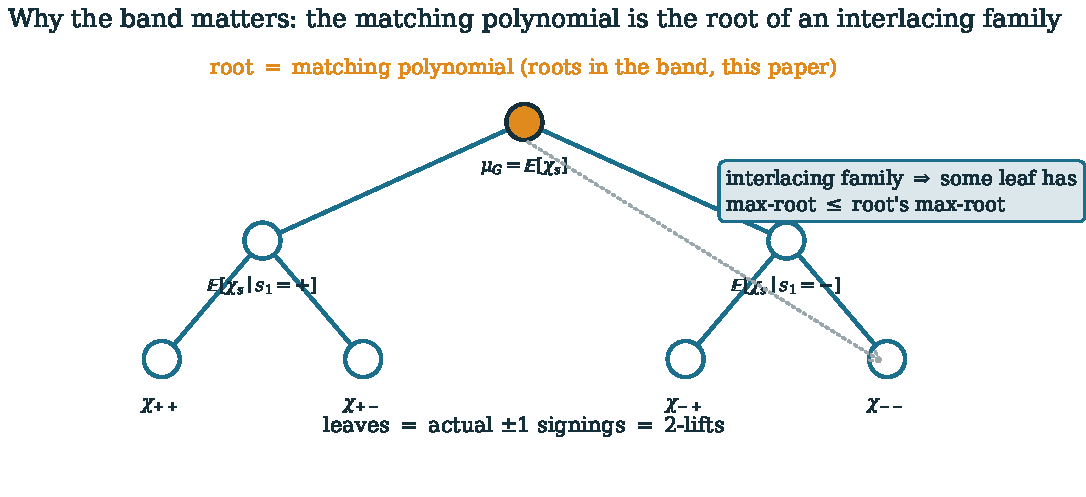
\includegraphics[width=0.86\textwidth]{fig7_interlacing.pdf}
  \caption{D\'onde se sit\'ua este teorema en el argumento de Marcus--Spielman--%
  Srivastava. Fijar los signos de las aristas uno a uno construye un \'arbol binario
  de polinomios caracter\'isticos esperados condicionados; su raíz es el polinomio
  de emparejamientos---cuyas ra\'ices este art\'iculo confina a la banda---y sus
  hojas son los signados $\pm1$ reales, es decir, los $2$-recubrimientos. Como los
  polinomios forman una \emph{familia entrelazada}, alguna hoja tiene su mayor
  ra\'iz no mayor que la del raíz: un promedio acotado fuerza un individuo bueno.
  Este art\'iculo certifica la raíz; el \'arbol en s\'i es trabajo futuro (P1).}
  \label{fig:interlacing}
\end{figure}

Tambi\'en pregunt\'e, con honestidad y c\'omputo exacto, si algo en este marco da
asidero al problema \emph{abierto} de los grafos de Ramanujan no bipartitos de todo
grado~\cite{LevinSurvey}. No lo da, y la obstrucci\'on es mec\'anica. El m\'etodo de
entrelazado controla un extremo del espectro porque el polinomio esperado
$\mathbb{E}[\operatorname{charpoly}(A_s)]=\mu_G$ tiene ra\'ices reales. El manejo
bilateral natural ser\'ia $\mathbb{E}[\operatorname{charpoly}(A_s^2)]$, cuya mayor
ra\'iz controlar\'ia $\max_i|\lambda_i|$---pero un c\'omputo simb\'olico directo
muestra que ese promedio \emph{no} tiene ra\'ices reales en general (tiene, por
ejemplo, cero ra\'ices reales para $K_{3,3}$). La linealidad que hace especial al
polinomio de emparejamientos no sobrevive al cuadrado. Lo reporto como resultado
negativo: aqu\'i no hay grieta f\'acil, consistente con la reputaci\'on del problema.

% ===============================================================
\section{Implicaciones}
\label{sec:implications}

\emph{M\'as all\'a del teorema mismo, ¿qu\'e deja esta demostraci\'on para que otro
lo use?}

\paragraph{Bloques reutilizables y certificados.} Nuevos en Mathlib y no
espec\'ificos de emparejamientos: \lean{collatzWielandt}, una cota de autovalores de
Gershgorin ponderado construida con los ingredientes de
\lean{Matrix.eigenvalue\_mem\_ball}; el predicado \lean{BoundedBy} con clausura bajo
divisores y productos y \lean{RealRooted.of\_dvd}; y dos hechos limpios sobre
distancias en \'arboles---los vecinos difieren en distancia-al-raíz por uno (v\'ia
bipartici\'on), a lo sumo un vecino est\'a m\'as cerca (v\'ia unicidad de
caminos)---que cualquier argumento sobre \'arboles con raíz en \lean{SimpleGraph}
puede reutilizar.

\paragraph{Alcance entre campos, y c\'omo sirve el artefacto a cada uno.}
Heilmann--Lieb est\'a en un cruce de caminos, y una versi\'on verificada es \'util de
forma distinta en cada uno. \emph{Mec\'anica estad\'istica / f\'isica
matem\'atica}: $\mu_G$ es la funci\'on de partici\'on mon\'omero--d\'imero, y la
banda es una regi\'on libre de ceros suya; la formalizaci\'on es un cimiento
verificado para argumentos de analiticidad al estilo Lee--Yang (energ\'ia libre sin
transici\'on de fase) en ret\'iculos de grado acotado. \emph{Teor\'ia espectral de
grafos e inform\'atica te\'orica}: el teorema es el motor anal\'itico tras los grafos
de Ramanujan, los expansores, la desaleatorizaci\'on y los c\'odigos correctores;
con la identidad de Godsil--Gutman (Paper~I) da los dos insumos verificados que una
demostraci\'on de existencia de expansores necesita, y un peldano concreto hacia un
Marcus--Spielman--Srivastava formalizado (P1). \emph{Combinatoria algebraica}: la
infraestructura reutilizable de raicicidad real y \lean{BoundedBy}---cerrada bajo
divisores y productos, alimentada por cotas espectrales sin entrelazado---se aplica a
cualquier cuesti\'on de polinomios de ra\'ices reales (log-concavidad de los $m_k$,
polinomios estables). \emph{Matem\'atica formal}: el polinomio de emparejamientos,
el \'arbol de caminos, una cota de autovalores de Gershgorin ponderado y dos lemas
de distancias en \'arboles son nuevos, de calidad Mathlib y contribuibles
\emph{aguas arriba}, donde bajan el coste de la siguiente formalizaci\'on espectral
o combinatoria. \emph{Teor\'ia de n\'umeros, por analog\'ia}: por la dualidad de la
Secci\'on~\ref{sec:duality} el mismo repositorio contiene el lado zeta de
Ihara / hip\'otesis de Riemann para grafos, as\'i que el artefacto es tambi\'en un
sustrato para una hip\'otesis de Riemann de grafos unificada y formalizada (P5).

\paragraph{Completando el programa del \'arbol de caminos.} Junto con el Paper~I, el
polinomio de emparejamientos, la identidad de Godsil--Gutman, el \'arbol de caminos,
la raicicidad real y la cota de las ra\'ices est\'an ahora verificados por m\'aquina.
Ning\'un asistente de pruebas, hasta donde s\'e, ten\'ia el polinomio de
emparejamientos ni ninguna mitad de Heilmann--Lieb antes de esta l\'inea de trabajo;
la afirmaci\'on de ``primero'' se apoya en una b\'usqueda en los ecosistemas
Lean/Mathlib, Isabelle/AFP y Coq/mathcomp (v\'ease la salvedad en la
Secci\'on~\ref{sec:intro}), y la matem\'atica es enteramente cl\'asica.

% ===============================================================
\section{Metodolog\'ia}
\label{sec:method}

\emph{¿Qu\'e ense\~n\'o construir esta demostraci\'on sobre c\'omo construir tales
demostraciones?} Como en el Paper~I, ejecut\'e un bucle de compilaci\'on-como-or\'aculo
con un sistema de IA (Claude, Anthropic): propon\'ia las definiciones y
demostraciones, el n\'ucleo de Lean verificaba o rechazaba cada una, y dimension\'e
el texto al veredicto del n\'ucleo. Para ser preciso sobre el reparto del trabajo,
ya que es justo preguntarlo: el asistente propuso esencialmente todas las
definiciones y \emph{scripts} de prueba en Lean y un primer borrador de este texto,
mientras que yo fij\'e el objetivo y la ruta, tom\'e las decisiones de dise\~no (la
elecci\'on del \'arbol de caminos, el peso local, el diagn\'ostico del muro de
elaboraci\'on), contrast\'e cada enunciado con la matem\'atica pretendida, y
respondo de todas las afirmaciones. La correcci\'on aqu\'i no descansa en la
confianza en el asistente: el n\'ucleo de Lean verific\'o cada l\'inea, una prueba
que rechaza nunca entra en el art\'iculo, y la no vacuidad de los enunciados la
atestigua \lean{\#print axioms} (Ap\'endice~\ref{sec:formal}). El asistente propone;
el n\'ucleo dispone.

Dos pr\'acticas fueron decisivas. Primero, la ruta hacia la cota se
\emph{des-arriesg\'o num\'ericamente antes de tocar Lean}: un breve estudio en
SageMath fij\'o qu\'e invariante inductivo cierra (un cociente plano por v\'ertice
falla en grafos con ciclos; el peso de \'arbol con raíz cierra exactamente en el
borde de la banda), de modo que la formalizaci\'on persigui\'o una ruta que ya se
sab\'ia que funcionaba---el peso local de la Secci\'on~\ref{sec:weight} surgi\'o
as\'i. Segundo, tras completar la prueba apliqu\'e la misma disciplina de
falsaci\'on \emph{a mis propias conclusiones}, buscando deliberadamente un teorema
nuevo en la vecindad, y reporto el resultado honesto de la
Secci\'on~\ref{sec:context}: el territorio es cl\'asico y est\'a ocupado, y la
\'unica sonda prometedora la mat\'o un c\'omputo. La aportaci\'on es una
formalizaci\'on verificada, enunciada hasta la frontera exacta de lo que el n\'ucleo
comprob\'o, con los negativos reportados con la misma claridad que los positivos.

% ===============================================================
\section{Trabajo relacionado}
\label{sec:related}

La matem\'atica es cl\'asica. Heilmann--Lieb~\cite{HeilmannLieb1972} es el objetivo;
la ruta del \'arbol de caminos y la cota espectral del bosque son de
Godsil~\cite{Godsil1981Matchings,Godsil1993}, con la cota elemental del radio
espectral de \'arboles tambi\'en en Stevanovi\'c~\cite{Stevanovic2003}; el teorema
es la mitad anal\'itica de Marcus--Spielman--Srivastava~\cite{MSS2015a}; el cuadro de
la funci\'on de Green de la Secci\'on~\ref{sec:duality} es
Abert--Csikvari--Frenkel--Kun~\cite{AbertCsikvariFrenkelKun2016} y su cara de zeta de
Ihara es Terras~\cite{Terras2011}. En el lado de la formalizaci\'on,
Mathlib~\cite{Mathlib2020} provee grafos simples, paseos, caminos, el polinomio
caracter\'istico, el teorema espectral para matrices hermitianas y el teorema del
c\'irculo de Gershgorin, pero no el polinomio de emparejamientos (Paper~I), el
\'arbol de caminos, ni una cota de emparejamientos \lean{BoundedBy} / Gershgorin
ponderado (este art\'iculo). No conozco tratamiento previo verificado por m\'aquina
de Heilmann--Lieb.

% ===============================================================
\section{Preguntas abiertas}
\label{sec:open}

Una formalizaci\'on est\'a tan viva como las preguntas que deja por hacer a
continuaci\'on. Dejo seis, ordenadas de la m\'as alcanzable a la m\'as especulativa;
cada una nombra una tensi\'on que no pude resolver aqu\'i.

\begin{enumerate}\itemsep3pt
\item[\textbf{P1}] \emph{(El siguiente peldano.)} Los dos insumos anal\'iticos de
  Marcus--Spielman--Srivastava est\'an ahora formalizados---el polinomio
  caracter\'istico esperado con signos \emph{es} $\mu_G$ (Paper~I) y sus ra\'ices
  est\'an en la banda (este art\'iculo). ¿Cu\'al es el \emph{menor} paso adicional
  que da la primera demostraci\'on verificada de que existen grafos de Ramanujan
  bipartitos de todo grado---el argumento de existencia de familias entrelazadas, o
  la correspondencia signado/$2$-recubrimiento?
\item[\textbf{P2}] \emph{(El m\'as dif\'icil.)} Mostr\'e que el manejo bilateral
  obvio $\mathbb{E}[\operatorname{charpoly}(A_s^2)]$ no tiene ra\'ices reales.
  ¿Existe \emph{alg\'un} polinomio, lineal en una estructura aleatoria
  combinatoria, cuya mayor ra\'iz controle $\max_i|\lambda_i|$ y siga teniendo
  ra\'ices reales? Un ``s\'i'' es una ruta hacia el problema abierto de Ramanujan no
  bipartito; este art\'iculo solo demuestra que el candidato obvio es un ``no''.
\item[\textbf{P3}] \emph{(Finura local.)} El peso local por arista da la cota
  $\sqrt{d_u-1}+\sqrt{d_v-1}$, estrictamente mejor que $2\sqrt{\Delta-1}$ en
  \'arboles irregulares. ¿Se traduce esa finura en un enunciado \'util sobre grafos
  irregulares---un umbral de expansi\'on irregular, o un an\'alogo irregular de la
  hip\'otesis de Riemann de grafos por el cuadro de Ihara--Bass con $Q=D-I$?
\item[\textbf{P4}] \emph{(Barato, no solo sobrevivible.)} El muro de elaboraci\'on de
  los caminos $\Sigma$ se cruz\'o con una cirug\'ia de irrelevancia de instancia,
  pero el coste sigue ah\'i. ¿Puede reprobarse la invariancia de $\mu$ bajo
  isomorfismo \lean{whnf}-libre (v\'ia su biyecci\'on de conjunto de aristas en vez
  de un conteo de emparejamientos por grado), volviendo barata la maquinaria del
  \'arbol de caminos para cualquier desarrollo futuro?
\item[\textbf{P5}] \emph{(Una variable, un teorema.)} La dualidad $u=1/R$ pone el
  lado de los emparejamientos y el de la zeta de Ihara sobre una sola variable
  uniformizante, compartiendo el sustrato \lean{BoundedBy} en un repositorio.
  ¿Existe un \'unico enunciado formalizado del que ca\'igan como lecturas tanto la
  banda de Ramanujan (emparejamientos) como la hip\'otesis de Riemann de grafos
  (zeta)?
\item[\textbf{P6}] \emph{(Para el f\'isico.)} $\mu_G$ es la funci\'on de partici\'on
  mon\'omero--d\'imero, y la banda es una regi\'on libre de ceros suya. ¿Tiene la
  raicicidad real y la banda verificadas por m\'aquina una consecuencia que un
  f\'isico estad\'istico querr\'ia---analiticidad de la energ\'ia libre, una
  ausencia de transici\'on de fase al estilo Lee--Yang---ahora ella misma
  verificable por m\'aquina?
\end{enumerate}

% ===============================================================
\section{Conclusi\'on}

El Paper~I pregunt\'o c\'omo podr\'ia verificarse por m\'aquina un enunciado de
raicicidad real sobre un grafo arbitrario, propuso el \'arbol de caminos de Godsil
como respuesta, y lo dej\'o como invitaci\'on expl\'icita. Este art\'iculo acepta la
invitaci\'on y termina el trabajo: construye el \'arbol de caminos, demuestra la
identidad del bosque y la divisibilidad---cruzando el \'unico muro de elaboraci\'on
que hab\'ia detenido al borrador---y demuestra la cota de Ramanujan a partir de una
estimaci\'on de Gershgorin ponderado alimentada por un peso geom\'etrico de \'arbol
y dos hechos sobre distancias en un \'arbol. El resultado es el teorema de
Heilmann--Lieb, ambas mitades, \lean{sorry}-libre, hasta la frontera exacta
$\Delta\ge2$ donde se cumple. Nada de la matem\'atica es nuevo; la aportaci\'on es
que ahora est\'a verificada donde no pude hallar formalizaci\'on previa, y que la
piedra nombrada al final del Paper~I queda puesta.

Y el viaje termina donde empez\'o: con un solo n\'umero. La cantidad
$2\sqrt{\Delta-1}$ marc\'o primero el borde de la analiticidad de un gas reticular;
reapareci\'o como el radio espectral de un \'arbol infinito, luego nombr\'o los
grafos de Ramanujan, luego rigi\'o la l\'inea cr\'itica de la funci\'on zeta de un
grafo. Este art\'iculo deja constancia, en una forma que una m\'aquina ha verificado
desde los axiomas, de que el mismo n\'umero acota tambi\'en los emparejamientos de
todo grafo finito. Un n\'umero, cuatro veces---y, para esta \'ultima lectura, ahora
fuera de duda.

\paragraph{Artefactos y reproducibilidad.} Todas las fuentes Lean son
\lean{sorry}-libres y dependen solo de los tres axiomas est\'andar
(Ap\'endice~\ref{sec:formal}, Tabla~\ref{tab:results}). La compilaci\'on usa la
cadena \lean{leanprover/lean4:v4.30.0-rc2} contra un clon de Mathlib;
\lean{lake build MSS} comprueba el desarrollo (salida~0), y la no vacuidad de cada
teorema cabecera se reproduce con un fichero de tres l\'ineas---\lean{import
MSS.HeilmannLiebBound}; \lean{open SimpleGraph}; \lean{\#print axioms
matchingPoly\_bounded}---ejecutado con \lean{lake env lean}. El estado exacto que
acompa\~na a este art\'iculo queda fijado por su DOI de Zenodo; las fuentes y las
comprobaciones num\'ericas en SageMath est\'an en:
\begin{center}
\url{https://github.com/karlesmarin/godsil-gutman-lean}
\end{center}

% ===============================================================
\appendix
\section{Enunciados formales, literales}
\label{sec:formal}

\emph{¿Dice el enunciado en Lean el teorema, o algo m\'as d\'ebil?} Es la primera
pregunta que un lector cuidadoso de una formalizaci\'on deber\'ia hacer, y merece
respuesta directa. Abajo est\'an las definiciones que cargan el peso y las dos
firmas cabecera, transcritas de la fuente (identificadores en tipograf\'ia de
m\'aquina, los operadores Unicode renderizados en matem\'aticas). La raicicidad real
es escindir sobre $\R$; el predicado de banda es la raicicidad real \emph{y} la cota
de magnitud sobre toda ra\'iz---as\'i que las conclusiones son los enunciados
genuinos, no debilitamientos.

\begin{tcolorbox}[colframe=ggteal,colback=ggband!25,arc=2pt,boxrule=0.8pt,left=8pt,right=8pt]
\ttfamily\small\setlength{\parindent}{0pt}
def RealRooted (p : Polynomial $\R$) : Prop := p.Splits\\[2pt]
def BoundedBy (p : Polynomial $\R$) (B : $\R$) : Prop :=\\
\hspace*{1.5em}RealRooted p $\wedge$ $\forall$ x : $\R$, p.IsRoot x $\rightarrow$ |x| $\leq$ B\\[2pt]
def bruhatTitsBound (k : $\mathbb{N}$) : $\R$ := 2 * Real.sqrt (k - 1 : $\R$)\\[4pt]
def matchingPoly : Polynomial $\R$ :=\\
\hspace*{1.5em}$\sum$ k $\in$ Finset.range (Fintype.card V / 2 + 1),\\
\hspace*{3em}Polynomial.C ((-1 : $\R$)\^{}k * (G.matchingNumber k : $\R$))\\
\hspace*{3em}* Polynomial.X\^{}(Fintype.card V - 2 * k)\\[6pt]
theorem matchingPoly\_realRooted (G : SimpleGraph V) [DecidableRel G.Adj] :\\
\hspace*{1.5em}MSS.RealRooted G.matchingPoly\\[4pt]
theorem matchingPoly\_bounded (G : SimpleGraph V) [DecidableRel G.Adj] ($\Delta$ : $\mathbb{N}$)\\
\hspace*{1.5em}(h$\Delta$ : 2 $\leq$ $\Delta$) (hdeg : $\forall$ v, G.degree v $\leq$ $\Delta$) :\\
\hspace*{1.5em}BoundedBy G.matchingPoly (bruhatTitsBound $\Delta$)
\end{tcolorbox}

\noindent Ning\'un teorema es vacuo. Un enunciado de la forma
``$\dots\lor\mathrm{True}$'' tambi\'en ser\'ia \lean{sorry}-libre, as\'i que la
ausencia de \lean{sorry} es necesaria pero no suficiente; son las conclusiones
\emph{expl\'icitas} de arriba---\lean{RealRooted} y \lean{BoundedBy} con las
definiciones mostradas---las que descartan la vacuidad. Para cada teorema cabecera,
\lean{\#print axioms} devuelve exactamente
\lean{[propext, Classical.choice, Quot.sound]} (sin \lean{sorryAx}), y la biblioteca
\lean{MSS} completa compila (\lean{lake build MSS}, salida~0) bajo la cadena
\lean{leanprover/lean4:v4.30.0-rc2} contra un clon local de Mathlib.

\bibliographystyle{plain}
\bibliography{references}

\end{document}
